\documentclass[11pt, a4paper, oneside]{book}
\usepackage[utf8]{inputenc}
\usepackage{graphicx}
\usepackage{geometry}
\usepackage{titlesec}   
\usepackage{anyfontsize}
\usepackage{lipsum}
\usepackage{amsmath}
\usepackage[colorlinks=true, allcolors=blue]{hyperref}
\usepackage{float}

% Márgenes
\geometry{
    left=3cm,
    right=3cm,
    top=3cm,
    bottom=3cm,
}

% Formato del título de capítulos
\titleformat{\chapter}[display]
{\bfseries\centering}
{\Large Capítulo \thechapter}
{0pt}
{\Huge}
[\vspace{3ex}]
\titlespacing{\chapter}{0pt}{0em}{3em}


\begin{document}

\begin{titlepage}
    \centering
    
    % Línea superior
    \rule{\textwidth}{1.5pt}\\[0.5cm]
    
    % Título principal
    \textsc{\Huge Reporte de Documentación del}\\[0.3cm]
    \textsc{\Huge Proyecto Trueque Verde}\\[0.8cm]
    
    % Línea inferior
    \rule{\textwidth}{1.5pt}\\[1cm]
    
    % Área académica
    \large INSTITUTO TECNOLOGICO DE MATAMOROS \\[0.5cm]
    Ingenieria en Sistemas Computacionales\\[1cm]
    
    % Logo
    \IfFileExists{Pictures/iitk_logo.png}{
        
\includegraphics[width=0.3\textwidth]{Pictures/iitk_logo.png}
    }{\vspace{1.5cm}}
    \\[0.5cm]

    \textsc{Programación FrontEnd}\\[0.5cm]

    \Large\textbf{AUTORES }\\[0.5cm]
    
    {\large 
      \begin{tabular}{c}
        Marcos Iván Jiménez de la Cruz 21260170\\[0.3cm]
        Denes Ulises Mireles Rodríguez 21261105\\[0.3cm]
        Daniela Juan Hipólito 21260145\\[0.3cm]
        Esmeralda Teodoro Soreano 20260223\\[0.3cm]
        Juan Felipe Ávalos Pérez 21260130\\[0.3cm]
        Ernesto Vázquez Ramírez 21260181\\
      \end{tabular}
    \par}
    \vspace{1cm}
    
    \textsc{Docente}\\[0.2cm]
    \large Anabel Pineda Briseño  \\[1cm]        

    \large Marzo 2025
\end{titlepage}


\renewcommand{\contentsname}{Índice} 
\tableofcontents
\newpage
\chapter{Introducción}

\noindent El proyecto Trueque Verde surge con la finalidad de fomentar el intercambio de bienes y servicios de manera sostenible, promoviendo una economía colaborativa que incentive el cuidado del medio ambiente. En un contexto donde la responsabilidad social y el compromiso ecológico cobran cada vez más relevancia, esta plataforma se plantea como una solución integral para conectar a usuarios interesados en el intercambio responsable, facilitando tanto la comunicación como la gestión de transacciones de forma segura y amigable.

El desarrollo del proyecto se ha dividido en diversas áreas de trabajo, en las que cada equipo se ha encargado de implementar componentes específicos. Entre ellos se destacan la creación de interfaces de registro, catálogos de productos, sistemas de mensajería y mapas interactivos, tanto para plataformas web como móviles. En este sentido, el equipo 8 ha asumido la responsabilidad de recopilar y documentar de manera uniforme todos los aportes referentes al FrontEnd, con el objetivo de garantizar coherencia, facilidad de uso y mantenimiento a futuro.

Este reporte de documentación tiene como propósito describir detalladamente la estructura, diseño y funcionalidades implementadas en el FrontEnd de Trueque Verde. A través de esta guía, se busca proporcionar una visión clara y precisa de los lineamientos adoptados, los retos enfrentados y las soluciones propuestas durante el desarrollo. Además, se pretende servir como herramienta de referencia para futuros procesos de evaluación y mejora del sistema, contribuyendo al fortalecimiento de la plataforma como un recurso innovador y escalable en el ámbito del intercambio sostenible.

%Esmeralda PARTE EQUIPO 2

\chapter{Implementación de la interfaz de registro}

En este capítulo, se presentan los principales lineamientos y estrategias empleadas en el desarrollo de la interfaz de usuario, abordando desde la estructura de las vistas hasta los principios de diseño que rigen la plataforma. Se detallan aspectos clave como la disposición de los elementos en la pantalla de inicio de sesión, la organización del formulario de registro y las técnicas utilizadas para lograr una experiencia de usuario óptima.


A través de esta documentación, se proporciona una visión clara del enfoque adoptado en la construcción del FrontEnd, con el objetivo de asegurar coherencia visual, facilidad de uso y escalabilidad futura.


    \section{Login}
    El componente Login maneja la autenticación de usuarios existentes. Proporciona un formulario con validación en tiempo real, permitiendo a los usuarios ingresar su correo electrónico y contraseña. También incluye una opción \textquotedblleft{}Recuérdame\textquotedblright{} para mantener la sesión activa. Además, cuenta con enlaces para redirigir a la página de registro o a la recuperación de contraseña.

\begin{figure}[H]
    \centering
\includegraphics[width=9cm, height=8cm]{Pictures/1_Inicio de sesión.png}
    \caption{\label{fig:frog}Inicio de sesión.}

\end{figure}
    
    \section{Registro}
    El componente Register gestiona el registro de nuevos usuarios. Utiliza un formulario dividido en dos secciones para facilitar la captura de información personal y de cuenta. Además, permite la carga de una foto de perfil y aplica validaciones completas para asegurar la correcta entrada de datos.
    
    \begin{figure}[H]
    \centering
    \includegraphics[width=1.10\linewidth]{Pictures/2_Registro de sesión.png}
    \caption{\label{fig:frog}Formulario de registro.}
    \end{figure}

    \vspace{3cm}

        
    \section{Estructura Visual}
    AuthLayout proporciona una estructura visual consistente para las páginas de autenticación. Su diseño es responsivo, incluye un logo centralizado y un contenedor con sombras. Además, permite personalizar los títulos y descripciones de cada página.
    


    \section{Recuperación de Contraseña}
    El componente ForgotPassword permite a los usuarios recuperar el acceso a sus cuentas. Consiste en un formulario simple donde se solicita el correo electrónico registrado. Posteriormente, se envía un enlace de recuperación y se muestra un mensaje de estado al usuario.
    
    \begin{figure}[H]
    \centering
    \includegraphics[width=1.10\linewidth]{Pictures/3_Recuperar contraseña.png}
    \caption{\label{fig:frog}Recuperación de contraseña.}
    \end{figure}

    \section{Inicio de Sesión y Gestión de Usuario}

El sistema actual incorpora un módulo robusto de autenticación, navegación segura y persistencia de sesión, orientado a ofrecer una experiencia fluida, segura y escalable. A continuación se detallan sus características funcionales y técnicas.

\subsection*{Autenticación Segura}

\begin{itemize}
    \item Validación de credenciales tanto en frontend como en backend mediante JWT.
    \item Almacenamiento local seguro de tokens, con control de expiración y limpieza automática.
    \item Opción de persistencia condicional mediante el selector ``Recuérdame''.
    \item Navegación basada en datos completos del usuario autenticado.
\end{itemize}

\subsection*{Experiencia de Usuario}

\begin{itemize}
    \item Interfaz accesible y responsiva, diseñada con componentes nativos.
    \item Indicadores visuales de carga e interacción inmediata.
    \item Estructura adaptada a pantallas de distintos tamaños.
\end{itemize}

\subsection*{Gestión de Estado y Navegación}

\begin{itemize}
    \item Manejo de usuario con \texttt{UserContext} y persistencia con \texttt{AsyncStorage}.
    \item Eliminación automática de datos obsoletos o sesiones inválidas.
    \item Navegación tipada con verificación estricta de tipos.
\end{itemize}

\subsection*{Compatibilidad y Patrones de Diseño}

\begin{itemize}
    \item Compatibilidad con:
        \begin{itemize}
            \item React Native 0.70.0
            \item React Navigation 6.0.0
            \item React Native Paper 5.0.0
        \end{itemize}
    \item Patrones utilizados:
        \begin{itemize}
            \item Context Pattern
            \item Repository Pattern
            \item Observer Pattern
            \item Factory Pattern
        \end{itemize}
\end{itemize}

\subsection*{Rendimiento Estimado}

\begin{itemize}
    \item Tiempo promedio de login: $\leq$ 2 segundos.
    \item Validación de token: $\leq$ 500 ms.
    \item Carga inicial del módulo: $\leq$ 1 segundo.
\end{itemize}














%DENES PARTE EQUIPO 2

\chapter{Implementación del catálogo de productos de intercambio}
\noindent 
\section{Frontend}

Las nuevas actualizaciones en cuestión del frontend del catálogo son del rediseño en cuestión del menú en donde se muestra el catálogo, se agregó un pequeño menú en la parte inferior y también el diseño e implementación del formulario de publicar un producto.

En la parte del catálogo está conformado por tres partes principalmente, el cuales son formPublicar.js, producto.js y screenCatalogo.js:\\

\textbf {ScreenCatalogo.js} \\
El componente App representa la pantalla principal de productos dentro de una aplicación de intercambio. Permite a los usuarios buscar productos, filtrarlos por categoría, ver detalles mediante un modal, y navegar a otras pantallas. Los productos se obtienen desde un servidor externo y se actualizan periódicamente.\\


\textbf {Funcionalidades Principales}
\begin{itemize}
\item Búsqueda en tiempo real por nombre del producto.
\item Filtro por categoría desde un menú desplegable.
\item Visualización de productos en tarjetas dentro de un FlatList.
\item Modal que muestra información detallada del producto mediante el componente Producto.
\item Actualización automática de productos cada 5 segundos desde el backend.
\item Carga de fuentes personalizadas (Poppins) usando expo-font.
\end{itemize}

\begin{center}
\textbf {Actualizaciones en el frontend del catalogo.}    
\end{center}

\begin{figure} [H]
    \centering
    \begin{minipage}{0.45\textwidth}
        \centering
        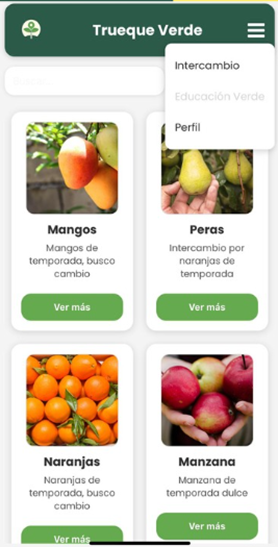
\includegraphics[width=\textwidth]{Pictures/Imagen4.png}
        \caption{Menu antes de las modificaciones.}
    \end{minipage}
    \hfill
    \begin{minipage}{0.40\textwidth} 
        \centering
        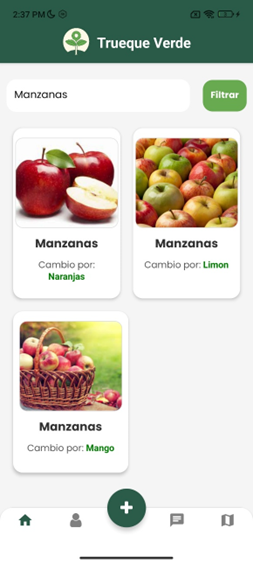
\includegraphics[width=\textwidth]{Pictures/Imagen5.png}
        \caption{Diseño actualizado.}
    \end{minipage}
\end{figure}

Como anteriormente se mencionó se cambió la parte donde se muestran los catálogos agregando un menú que permita al usuario moverse entra las diferentes vistas y poder publicar con esto se retiro el botón de publicar y el menú de la parte superior.

\newpage
\section{FormPublicar.js.}
El componente FormPublicar es un formulario que permite a los usuarios autenticados publicar productos para intercambio. Los usuarios deben proporcionar información como el nombre del producto, una descripción, fotos, lo que desean recibir a cambio, una categoría y su ubicación.

\textbf {Funcionalidades Principales}
\begin{itemize}
\item Captura de datos del producto: nombre, descripción, categoría y elemento deseado en intercambio.
\item Selección de múltiples imágenes desde la galería del dispositivo utilizando expo-image-picker.
\item Obtención de ubicación del usuario (opcional).
\item Envío de los datos y archivos al backend mediante axios.
\item Validación básica de campos y del estado de autenticación del usuario.
\item Feedback visual durante el envío de datos.\\
\end{itemize}

\textbf {Renderizado del Formulario}\\
\textbf {Incluye:}
\begin{itemize}
\item Campo de texto para nombre del producto.
\item Campo de texto para descripción (multilínea).
\item Botón para subir imágenes + vista previa de las imágenes seleccionadas.
\item Campo de texto para "cambio por".
\item Selector de categoría (Picker).
\item Texto de ubicación basada en userLocation o coordenadas por defecto.
\item Botón de envío que se desactiva mientras se procesa.
\end{itemize}

\newpage
\section{\textbf{Actualización del frontend del formulario de productos}}

Anteriormente no se contaba con el diseño ni con la funcionalidad del formulario destinado a la creación de publicaciones. Sin embargo, esta sección ya se encuentra completamente implementada. Ahora, los usuarios tienen la posibilidad de crear publicaciones en las que especifican los productos de su cosecha que desean intercambiar, así como aquellos que están buscando obtener a cambio. Este formulario incluye campos como el título, la descripción, imágenes, la categoría del producto, la ubicación y otros datos relevantes. Con esta implementación, se facilita la interacción entre los usuarios, promoviendo el intercambio directo de productos agrícolas y fomentando la colaboración dentro de la comunidad.

\begin{figure}[H]
    \centering
    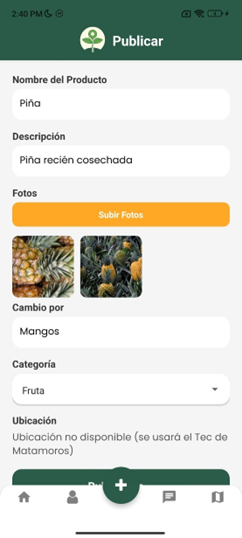
\includegraphics[width=0.40
    \linewidth]{Pictures/Imagen6.png}
        \caption{Imagen del acceso a Git}

\end{figure}

\newpage
\section{Producto.Js}

Este componente muestra los detalles de un producto en un modal: un carrusel de imágenes, información del intercambio, descripción, datos del dueño, ubicación, y un campo para enviar un mensaje al propietario para iniciar un chat.\\

\textbf {Funciones principales:}

\begin{itemize}
\item Visualización de imágenes: carrusel horizontal de imágenes del producto, ya sea desde URLs remotas o imágenes locales por defecto.
\item Envío de mensaje: permite al usuario interesado escribir y enviar un mensaje para iniciar una conversación con el propietario del producto.
\item Inicio de conversación: al presionar "Enviar", se crea (o reutiliza) una conversación y se redirige al usuario al chat correspondiente.
\item Visualización de detalles: se muestran la descripción del producto, información del propietario y ubicación.
\item Modal de cierre: puede cerrarse tocando el botón de cierre superior.
\end{itemize}

\section{\textbf {Backend}}
Para que funcione todo lo que se encuentra en las vistas del menú principal, el filtrado, la visualización del de producto y su publicación contamos con tres controladores los cuales son CategoryController, ItemController y PostController, junto a sus modelos Category, Item y Post. Algo que tomar en cuenta es que en todos los controladores manejan método index, store, show, update y destroy, pero en cada uno de los controladores funcionara de manera distinta.\\

\textbf {Controladores.}\\

\textbf {CategoryController.}\\
El controlador CategoryController tiene como propósito central gestionar todas las operaciones relacionadas con el modelo Category.\\

\textbf {Metodos.}\\

\textbf {Index:} El primer método del controlador es index(), que tiene como función devolver una lista completa de todas las categorías almacenadas en la base de datos. \\

\textbf {Store:} El siguiente método es store, que se encarga de crear una nueva categoría. Este método primero realiza una validación de los datos recibidos. Se asegura de que el campo name esté presente, sea una cadena y tenga una longitud máxima de 255 caracteres. Si los datos no cumplen con estas reglas, se devolverá automáticamente un error de validación.\\ 

\textbf {Show:} Después, se encuentra el método show, que recibe directamente una instancia del modelo Category gracias a la funcionalidad de route model binding de Laravel.\\

\textbf {Update:} El método update permite actualizar una categoría existente. \\

\textbf {Destroy:} El último método es destroy, que elimina la categoría proporcionada. \\

\textbf {ItemController.}
El controlador ItemController es responsable de gestionar todas las operaciones relacionadas con los items dentro del sistema.\\

\section{\textbf {PostController.}}

El controlador PostController, se encarga de gestionar las operaciones relacionadas con las publicaciones (posts) dentro de la aplicación. \\

\textbf {Métodos.}\\

\textbf {Index:} Este método se encarga de recuperar todos los posts existentes en la base de datos. \\

\textbf {Store:} Este es el método más complejo del controlador y tiene como objetivo crear una nueva publicación.\\

\textbf {Show:} Este método permite visualizar los detalles de un post en particular. Recibe un objeto Post gracias a la inyección automática de modelos de Laravel, y luego carga sus relaciones user e item para incluir la información completa relacionada.\\

\textbf {Update:} Este método se encarga de actualizar un post existente. Recibe los datos del request y los valida, permitiendo que muchos de los campos sean opcionales. Es decir, solo se actualizarán aquellos campos que estén presentes en el request y sean válidos.\\

\textbf {Destroy:} El propósito de este método es eliminar un post de la base de datos.\\

\textbf {Modelos}\\
Los controladores de esta aplicación trabajan directamente con los modelos para gestionar la información de la base de datos. Cada modelo representa una entidad con sus relaciones, y los controladores definen las operaciones que se pueden realizar sobre ellas.\\

\textbf {Item}\\
La función de category define una relación donde cada ítem pertenece a una sola categoría.\\

Por último, la función de posts indica que un ítem puede estar asociado a varios posts, es decir, un ítem puede aparecer en muchas publicaciones.\\

\textbf {Category}\\
En el arreglo protected fillable muestra que solo se tiene un campo asignable: el nombre de la categoría (por ejemplo: “Fruta”, “Planta”, etc.).\\

Mientras la función define que una categoría puede tener muchos ítems asociados.\\

\textbf {Post}\\
El arreglo permite asignar los siguientes datos al crear o actualizar un post:

\begin{itemize}
\item title: Título de la publicación.
\item content: Contenido o descripción.
\item image: Ruta(s) de la(s) imagen(es) asociada(s).
\item userid: ID del usuario que publicó.
\item itemid: ID del ítem relacionado.
\item statusid: Estado del post (pendiente, aprobado, etc.).
\item latitude, longitude: Coordenadas de ubicación.
\item greenpointd: Punto verde asociado (si existe).
\end{itemize}

La función de user relaciona el post con el usuario que lo creó.\\

La ultima función de Item relaciona el post con el ítem asociado (por ejemplo, una planta, fruta, etc.).\\


















%DANIELA EQUIPO 3_
\chapter{Implementación del sistema de intercambio}
\noindent
\section{Funcionalidades Clave} 

Solicitud de trueque: 

\begin{enumerate} 

    \item Botón para solicitar un intercambio, con un formulario donde se especifique qué se ofrece y qué se busca. 

 \item Validación automática para evitar duplicados o datos incompletos. 

\item Mensajería interna 

\item Sistema de chat para que los usuarios negocien detalles del trueque (cantidad, punto de encuentro, etc.). 

\end{enumerate} 

\section{ Formulario y Chat } 

\subsection{ Funcionalidades Principales} 

\begin{itemize} 

    \item Chat integrado: Permite a los usuarios ponerse de acuerdo fácilmente. 

\end{itemize} 

\begin{itemize} 

    \item Formulario de intercambio: Ayuda a registrar qué se ofrece, qué se busca a cambio, la ubicación y hasta agregar fotos. 

\end{itemize} 

\begin{itemize} 

    \item Diseño sencillo e intuitivo: La aplicación está pensada para que cualquiera pueda usarla sin problemas. 

\end{itemize} 

\subsection{Estructura} 

     Pantallas Principales: 

\begin{itemize} 

    \item Pantalla de inicio para explorar opciones de trueque  

\end{itemize} 

\begin{itemize} 

    \item Pantalla del chat para negociar intercambios  

\end{itemize} 


\vspace{3cm}
Se utilizo React Native junto con Expo para el
desarrollo y prueba de la aplicación, y NativeWind para estilizar las pantallas con clases
de Tailwind CSS, lo que nos permitido mantener un diseño uniforme y adaptable.
Adaptando esta configuración a nuestras pantallas, se visualizan de la siguiente forma.



\begin{itemize} 

    \item Formulario de Intercambios   

\end{itemize} 

\begin{figure}[H] 

\centering 

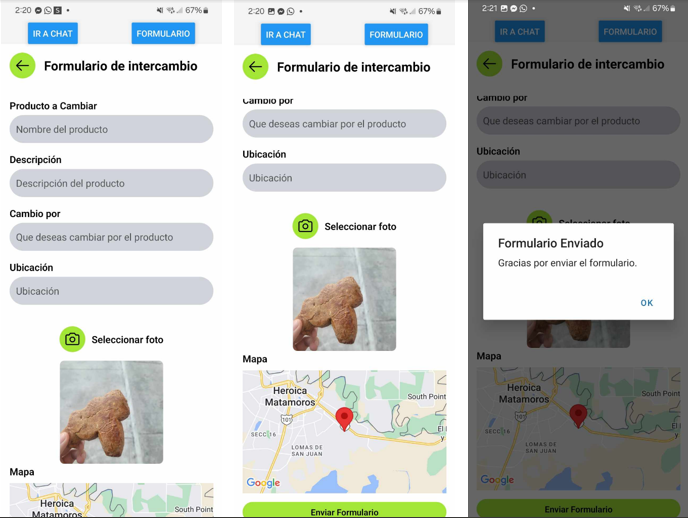
\includegraphics[width=0.75\textwidth]{Pictures/formularionuevo.png} 

\caption{Formulario} 

\end{figure} 

\begin{itemize} 
    


\chapter{Implementacion de la Base de Datos} 

 

\section{Sistema de Intercambio y Mensajes} 

 

Esta base de datos consta de varias tablas interrelacionadas, cuya función es gestionar y almacenar las solicitudes de trueques, las interacciones entre los usuarios, y el contenido de las conversaciones. A continuación se describen las principales tablas y sus campos: 

 

 

\begin{enumerate} 

    \item Tabla de Trueques:  

 

Esta tabla está diseñada para gestionar las solicitudes de trueque y almacenar la información relacionada con las transacciones entre usuarios.  Los campos que contiene son los siguientes: 

 

\begin{itemize} 

    \item Id Trueque: Un identificador único para cada solicitud de trueque. 

\end{itemize} 

\begin{itemize} 

    \item Id publicacion: Relaciona la solicitud con la publicación en la que se basa el trueque. 

\end{itemize} 

\begin{itemize} 

    \item Id usuario ofertante: Relaciona la solicitud con el usuario que realiza la oferta, referenciando a la tabla de usuarios para obtener su información. 

\end{itemize} 

\begin{itemize} 

    \item Descripción: Permite agregar una descripción detallada de la solicitud de trueque. 

\end{itemize} 

\begin{itemize} 

    \item Id status: Indica el estado del trueque, como activo, cerrado o rechazado. Este campo se relaciona con la tabla de estados (status). 

\end{itemize} 

\begin{itemize} 

    \item Latitud y Longitud: Guardan las coordenadas geográficas de la ubicación del trueque.  

\end{itemize} 

\begin{itemize} 

    \item Fecha: Indica la fecha y hora en que se creó la solicitud de trueque. 

\end{itemize} 

 

 

    \item Tabla de Conversaciones: 

 

Esta tabla es fundamental para almacenar las interacciones entre los usuarios que participan en una publicación, facilitando la comunicación. Los campos que componen esta tabla son: 

 

\begin{itemize} 

    \item  Id conversacion: Un identificador único para cada conversación.  

\end{itemize} 

\begin{itemize} 

    \item Id publicacion: Relaciona la conversación con una publicación específica 

\end{itemize} 

  \begin{itemize} 

      \item Id usuario creador: Hace referencia al usuario que creó la publicación, obteniendo su información desde la tabla de usuarios. 

  \end{itemize} 

  \begin{itemize} 

      \item Id usuario ofertante: Relaciona la conversación con el usuario interesado en la publicación. 

  \end{itemize} 

  \begin{itemize} 

      \item Id status: Indica si la conversación está activa o cerrada, relacionándose con la tabla de estados (status). 

  \end{itemize} 

  \begin{itemize} 

      \item Fecha: Registra la fecha y hora de creación de la conversación. 

  \end{itemize} 

 

 

\item Tabla de Mensajes: 

 

Esta tabla se utiliza para almacenar los mensajes enviados dentro de las conversaciones. Los campos que incluye son: 

 

\begin{itemize} 

    \item Id mensajes: Un identificador único para cada mensaje. 

\end{itemize} 

\begin{itemize} 

    \item Id conversacion: Relaciona el mensaje con una conversación específica. 

\end{itemize} 

\begin{itemize} 

    \item Idusuario: Hace referencia al usuario que envió el mensaje, obteniendo su información desde la tabla de usuarios. 

\end{itemize} 

\begin{itemize} 

    \item Contenido: Almacena el texto del mensaje 

\end{itemize} 

\begin{itemize} 

    \item Leído: Indica si el mensaje ha sido leído por el receptor 

\end{itemize} 

\begin{itemize} 

    \item Fecha: Registra la fecha y hora en que se envió el mensaje. 

\end{itemize} 

\end{enumerate} 

 

\begin{figure}[h!] 

\centering 

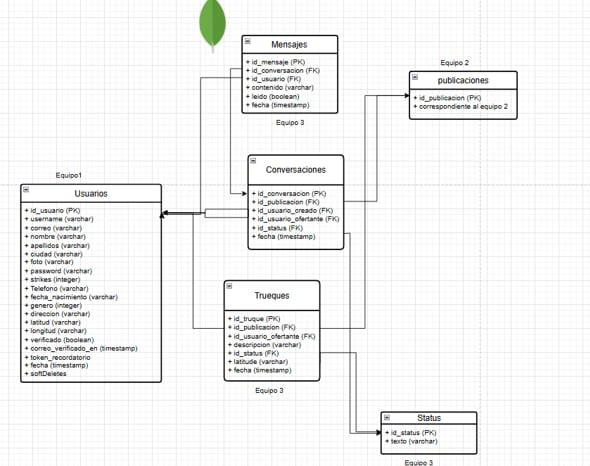
\includegraphics[width=\textwidth]{Pictures/tabalteam3.jpg} 

\caption{Diagrama} 

\label{fig:mi_imagen} 

\end{figure} 

 \vspace{3cm}

\section{Backend: Desarrollo de Tablas} 

los framgmentos de codigo  muestran el desarrollo de backend en Laravel que definen la estructura de las tablas "barters", "conversations" y "posts" dentro de una base de datos. 

\begin{itemize} 

    \item "barters" gestiona los intercambios entre usuarios, almacenando información sobre la oferta, el estado y la ubicación del trueque. 

\end{itemize} 

\begin{itemize} 

    \item "conversations" administra las interacciones entre usuarios en relación con una publicación, vinculando a los participantes y su estado. 

\end{itemize} 

 

\begin{itemize} 

    \item "posts" representa las publicaciones dentro de la aplicación, incluyendo detalles como título, contenido, imagen, ubicación y estado. 

 

\end{itemize} 

 

Cada tabla establece claves foráneas para mantener la integridad referencial en la base de datos, asegurando la correcta relación entre los distintos elementos del sistema. 


\end{itemize}


\section{Describcion del Modulo de Chat}

Dentro de la sección se muestra el backend donde se explica como funciona,los controladores que  se manejan son: ConversationController, MessageController y BarterController 

\subsection{Backend}
Controladores impelemtados:

\begin{enumerate}
    \item ConversationController:
    

Maneja las conversaciones entre usuarios. Incluye Funcionalidades para:

\begin{itemize}
    \item Listar todas las conversaciones en las que el usuario participa.
    \item Crear una nueva conversación entre dos usuarios para un post específico.
    \item Mostrar detalles de una conversación.
    \item Actualizar el estado de la conversación.
    \item Eliminar una conversación.
\end{itemize}
Este controlador usa autenticación para garantizar que solo los participantes puedan acceder a las conversaciones.


    \item MessageController:
   
    Administra los mensajes enviados dentro de las conversaciones.
    Permite:
     \begin{itemize}
         \item Consultar los mensajes de una conversación específica.
         \item Enviar un nuevo mensaje.
         \item Marcar un mensaje como leído.
         \item Eliminar un mensaje
        También incluye una función privada que valida si el usuario tiene acceso a la conversación.
     \end{itemize}

    \item BarterController:
    
   Controla las solicitudes de intercambio. Su funcionalidad principal es:

   \begin{itemize}
   \item  Registrar un nuevo trueque, validando los datos recibidos y actualizando el estado del producto relacionado para reflejar que está en proceso de intercambio
   \item También permite ver, actualizar o eliminar intercambios específicos del usuario autenticado.
   \end{itemize}
       
   \end{enumerate}

   \subsection{Frontend}
   
   \textbf{Pantalla de Producto} 
   
   
   En la pantalla de producto se habilito la opción para que el usuario interesado en un articulo pueda escribir un mensaje al propietario. una vez redactado y enviado, el sistema crea una conversación vinculada al producto y guarda el mensaje.

    
\begin{figure}[H]
 \centering
 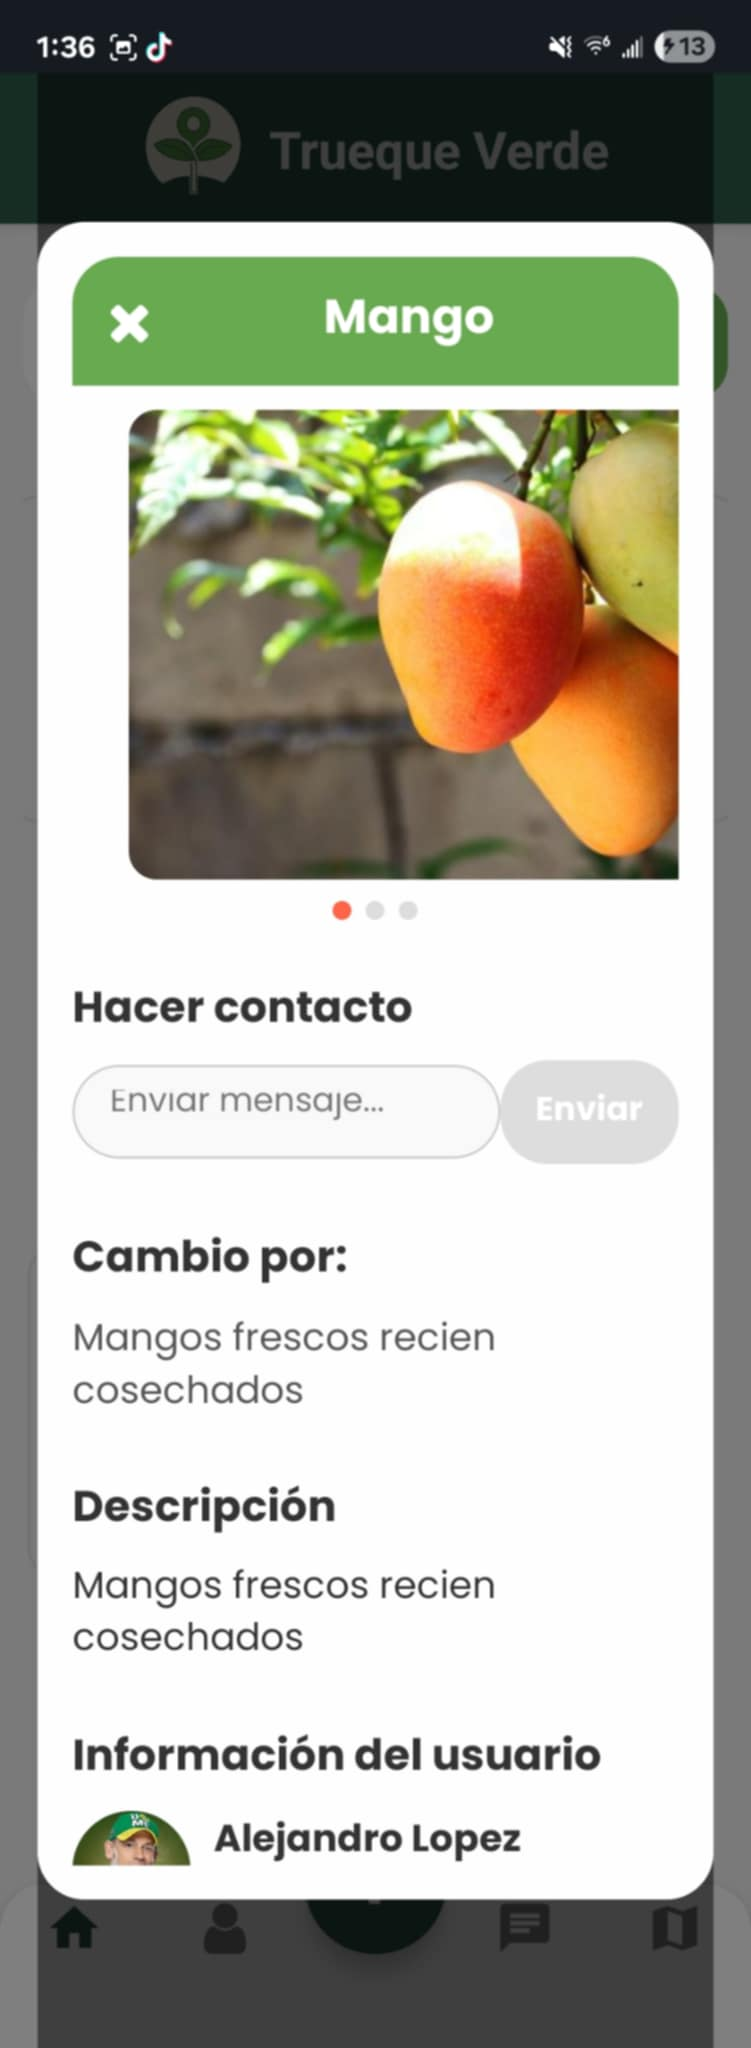
\includegraphics[width=0.28\textwidth]{Pictures/1.png}
          \caption{modal protocolo}
 
  \end{figure}


        \textbf{Pantalla de Chat}

La pantalla de chat fue diseñada para mostrar todos los mensajes de la conversación activa, distinguiendo visualmente cuáles fueron enviados por el usuario y cuáles por el interlocutor.



Se agrego un botón con un ícono de "+" que despliega un menú animado. Este menú ofrece funciones adicionales como acceder a un mapa o abrir el formulario de intercambio, en caso de que el usuario sea el ofertante del producto.



\begin{figure}[H]
    \centering
    \begin{minipage}[b]{0.25\textwidth}
        \centering
        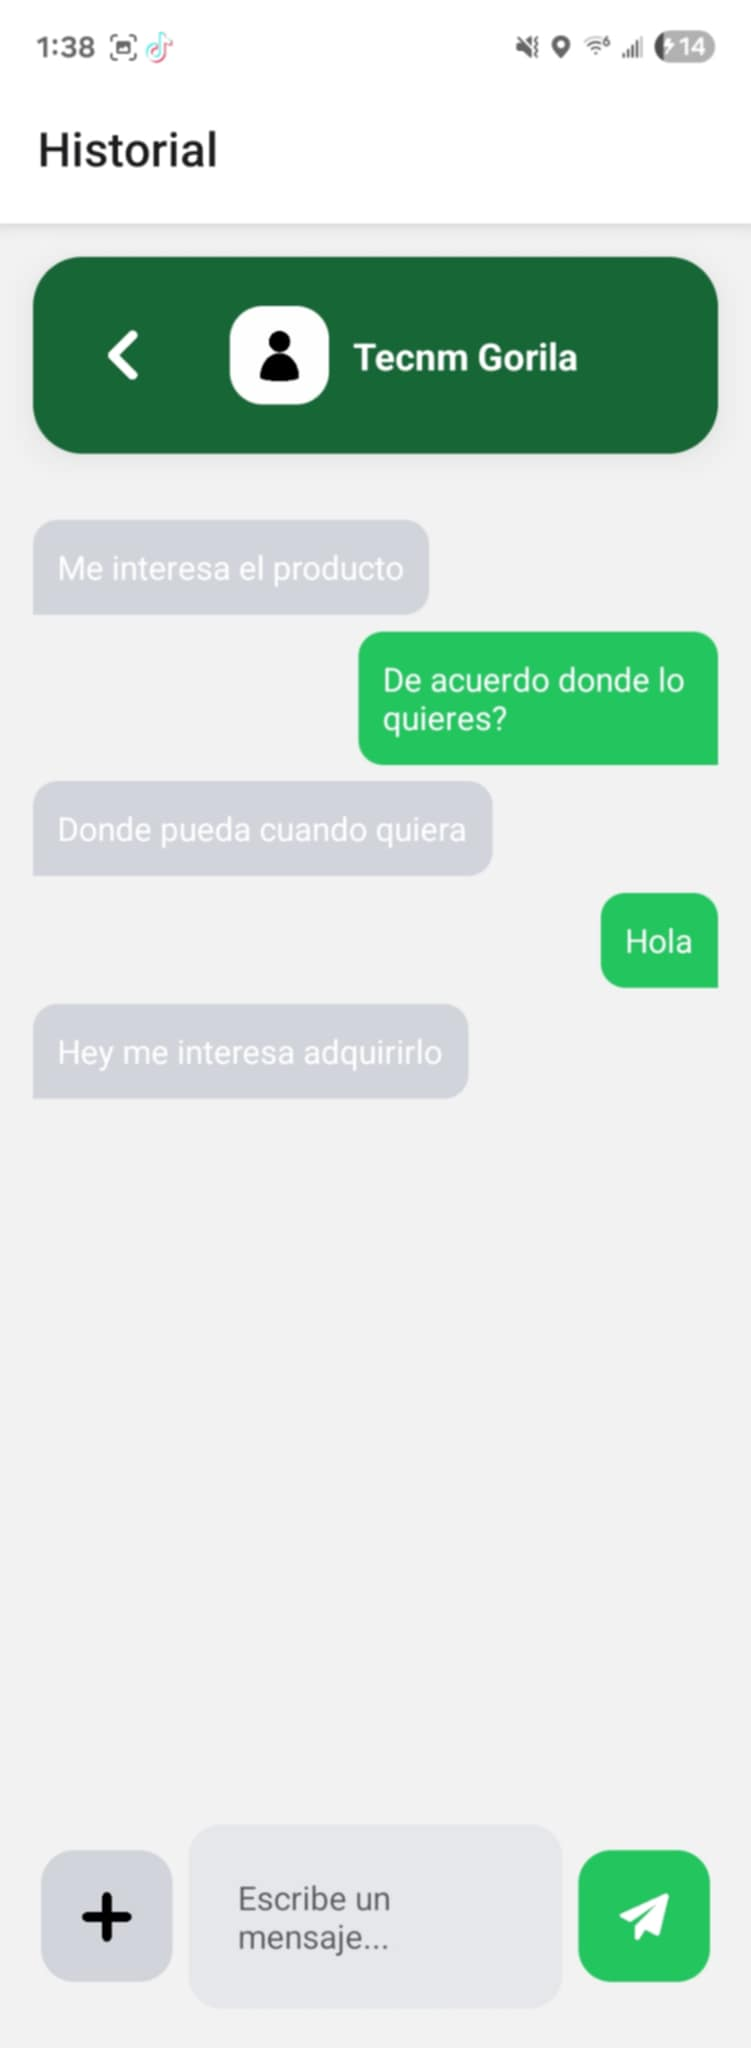
\includegraphics[width=\textwidth]{Pictures/3.png}
    \end{minipage}
    \hspace{0.03\textwidth} % Espacio entre imágenes
    \begin{minipage}[b]{0.3\textwidth}
        \centering
        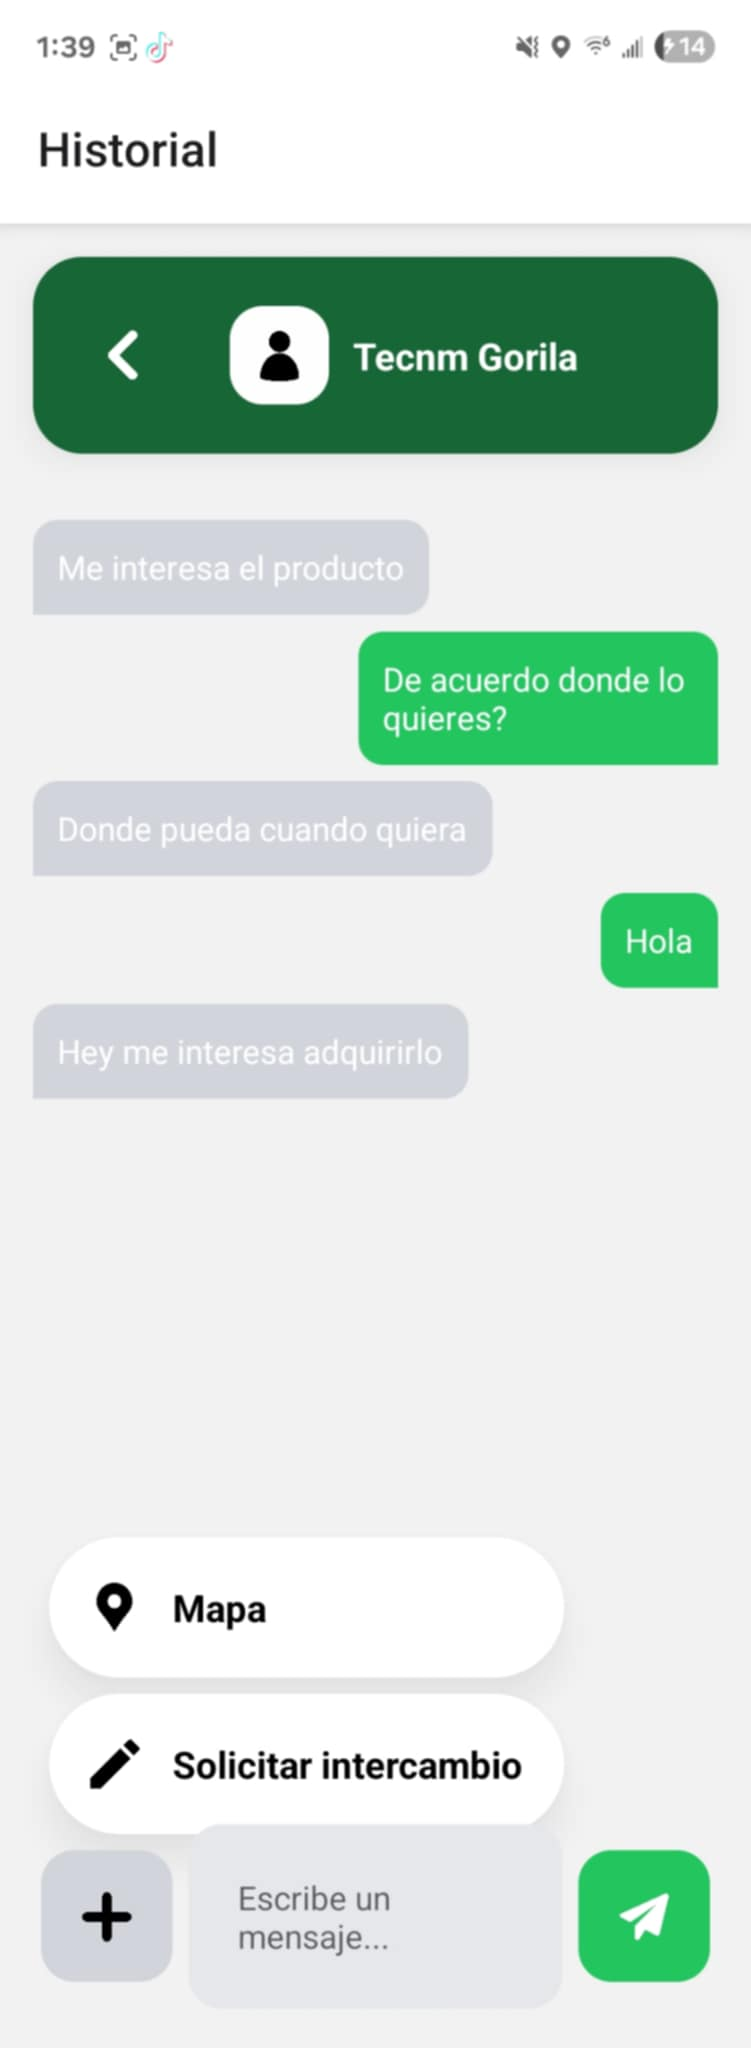
\includegraphics[width=0.85\textwidth]{Pictures/3-2.png}
    \end{minipage}
             \caption{Estilo de chat}
\end{figure}



 \textbf{Formulario de Trueque}

En cuanto al formulario de trueque, se implementó una pantalla que permite al usuario proponer un intercambio.
Esta pantalla contiene campos para ingresar el nombre del producto que ofrece, una descripción, el artículo 
que desea recibir a cambio y su ubicación. Se utiliza un mapa interactivo para facilitar la selección del 
lugar del intercambio. 

 \begin{figure}[H]
 \centering
 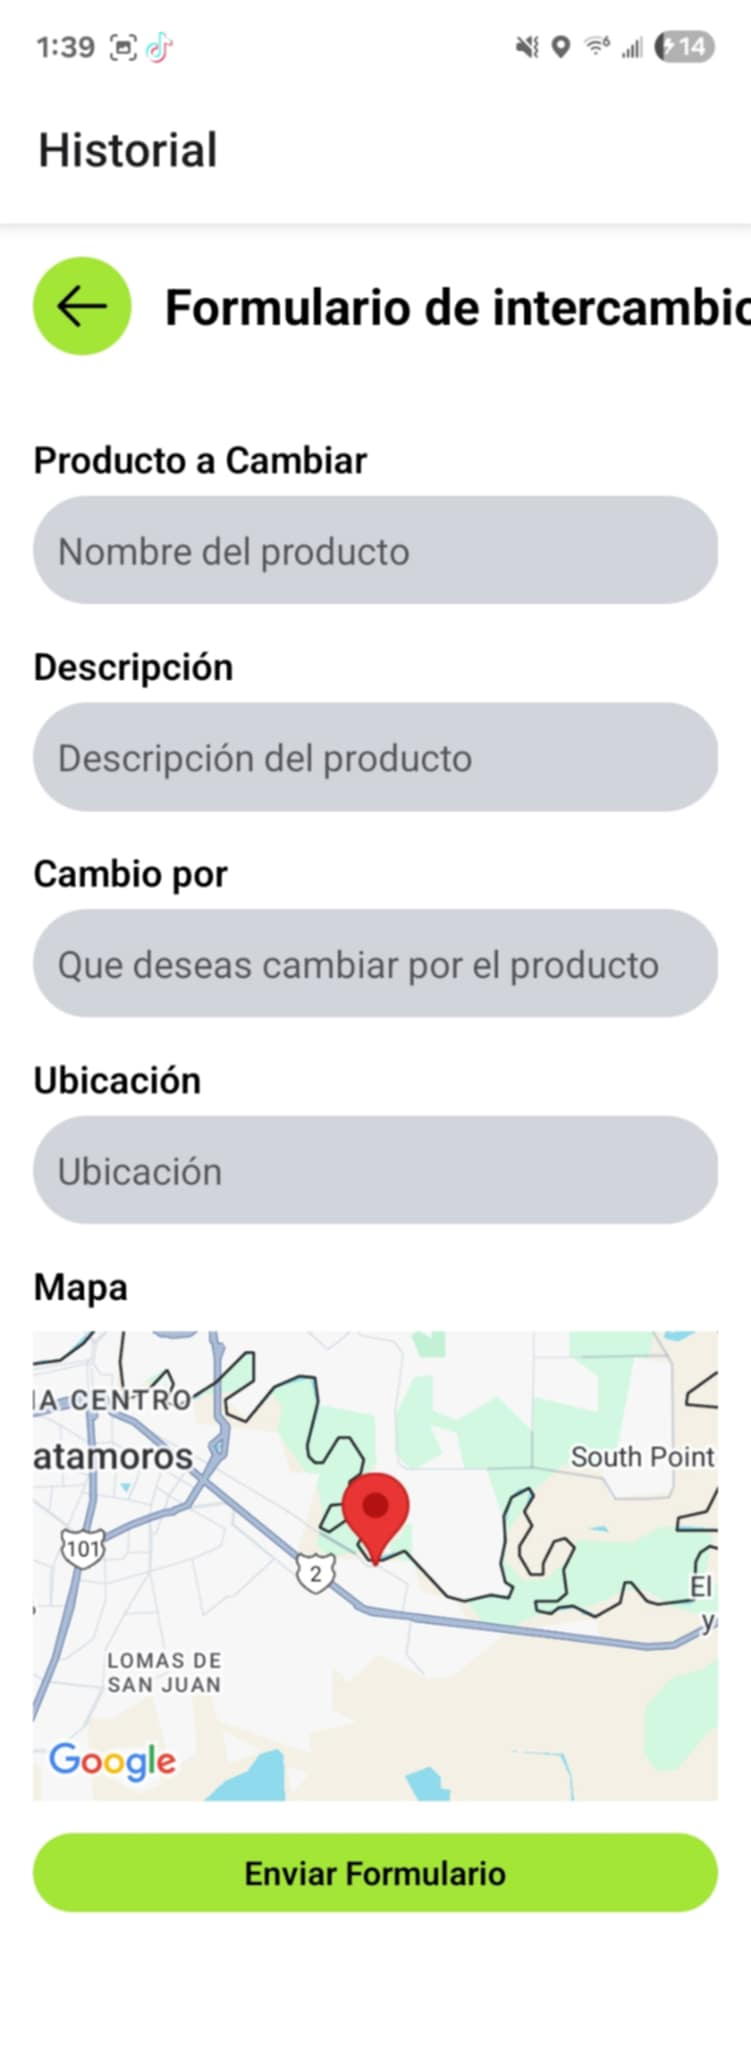
\includegraphics[width=0.2\textwidth]{Pictures/4.png}
 \caption{Diseño Formulario}
  \end{figure}

  

\textbf{Pantalla de lista de conversaciones}

Por último, la pantalla de lista de conversaciones permite al usuario ver todas las conversaciones activas en las que participa. En cada elemento de la lista se muestra el nombre del interlocutor, el último mensaje enviado, el título del producto asociado y la hora de la última actividad. Si el usuario selecciona una conversación, es redirigido automáticamente a la pantalla de chat correspondiente.


     

\begin{figure}[H]
\centering
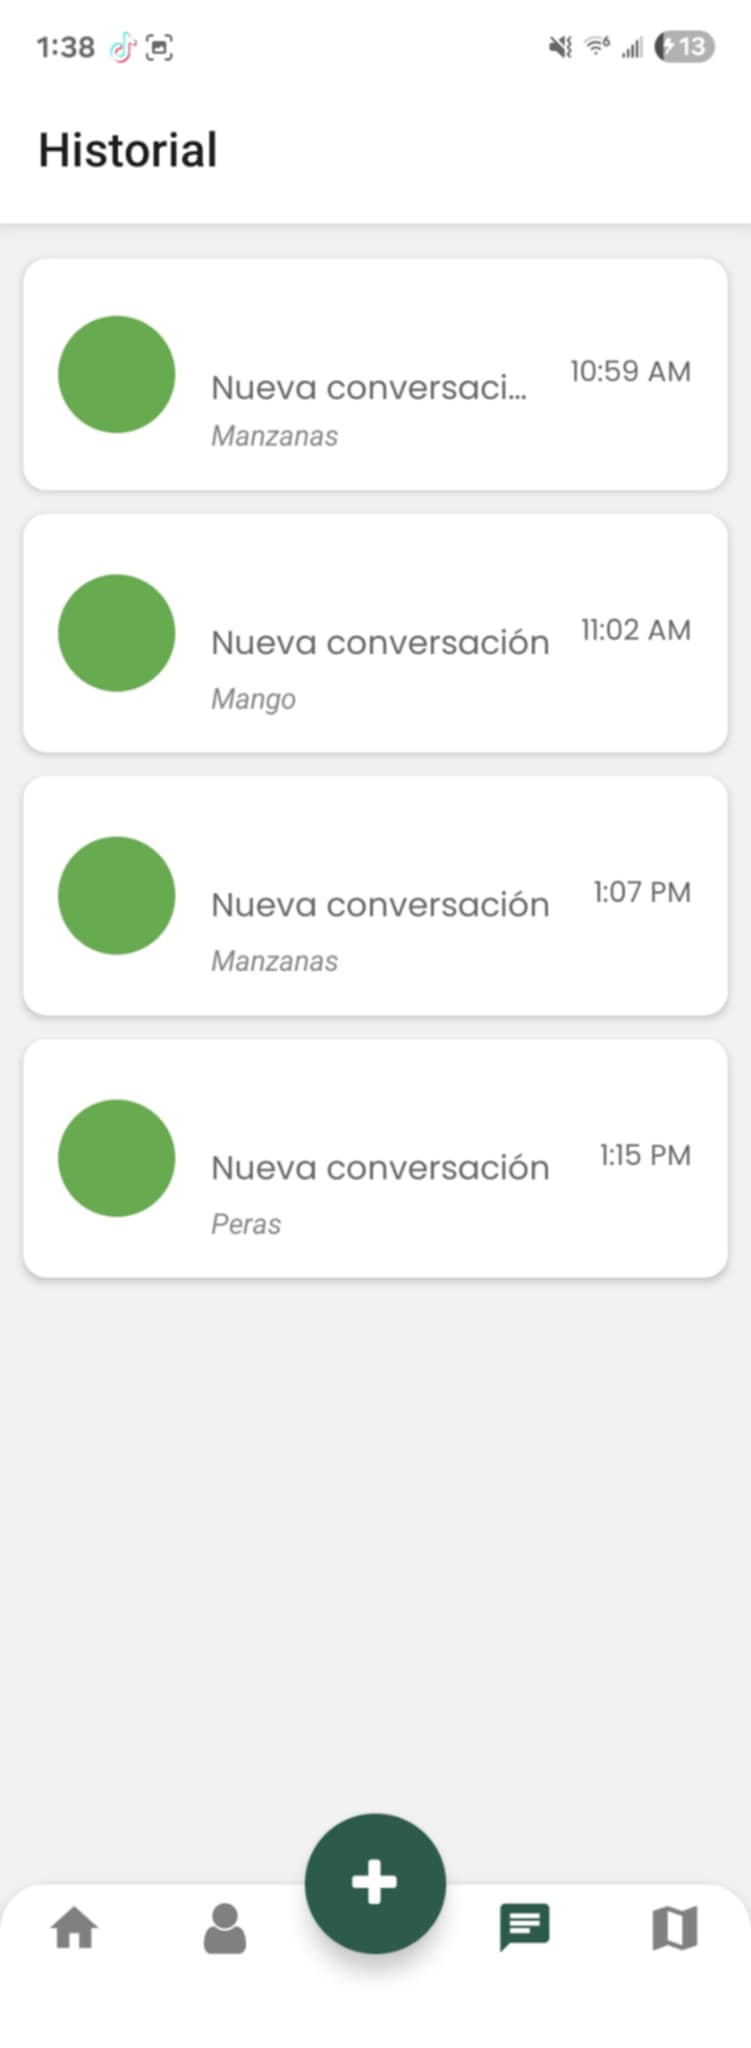
\includegraphics[width=0.3  4\textwidth]{Pictures/2.png}
         \caption{modal Historial}
\end{figure}



El proceso inicia cuando un usuario contacta al propietario de un producto desde su pantalla. Esto crea o reutiliza una conversación, permitiendo el intercambio de mensajes en un chat dinámico. Si el ofertante desea un trueque, puede enviar la solicitud desde el chat, la cual se valida y almacena en el backend, actualizando el estado del producto.



\chapter{Implementacion de Mapa Interactivo }

\noindent En esta sección se describe la funcionalidad de la pantalla de mapa dentro de la aplicación, la cual cumple un papel fundamental al permitir a los usuarios ubicar, visualizar y filtrar diferentes tipos de puntos relacionados con la oferta e intercambio de productos

 

\section{Pantalla de Mapa}

 

\noindent 
La pantalla de mapa tiene como objetivo principal facilitar la conexión entre usuarios mediante un sistema de geolocalización. Al ingresar, la aplicación solicita el permiso para acceder a la ubicación actual del usuario. Si se concede, el mapa se centra en su posición, y a partir de allí se muestran diferentes marcadores correspondientes a:

\begin{itemize}
    \item \textbf{Puntos verdes:} Lugares comunitarios o designados donde se pueden realizar intercambios de forma segura.
    \item \textbf{Publicaciones:} Productos específicos que otros usuarios han puesto a disposición, como frutas, semillas u otros alimentos.
\end{itemize}
Cada uno de estos elementos está representado con un ícono visual personalizado, lo que permite identificar fácilmente la categoría del producto.

\subsection{Interacción y Funciones Dinámicas}

El diseño del mapa no solo muestra ubicaciones, sino que ofrece una experiencia dinámica mediante un sistema de filtros inteligentes que permiten al usuario personalizar lo que desea ver:

\begin{itemize}
    \item \textbf{Filtro por tipo de marcador:} El usuario puede elegir entre ver todos los elementos, solo publicaciones o únicamente puntos verdes.

    \item \textbf{Filtro por categoría:} Se puede seleccionar una categoría específica (por ejemplo, semillas), lo que ajusta automáticamente los marcadores visibles a esa selección.

    \item \textbf{Filtro por distancia:} Un control deslizante permite definir un rango máximo en kilómetros, mostrando únicamente aquellos elementos que se encuentren dentro de ese radio.
\end{itemize}

Estos filtros están disponibles desde un menú desplegable accesible mediante un botón flotante en la pantalla.

Además, se incluye la posibilidad de actualizar manualmente la ubicación del usuario, en caso de que se haya desplazado o necesite refrescar los datos del mapa.

\subsection{Validaciones y Diseño}

Para garantizar una experiencia de usuario fluida y confiable, la pantalla de mapa incorpora diversas validaciones y consideraciones de diseño que contribuyen a su funcionalidad y atractivo visual.

\paragraph{Validaciones y manejo de errores:}
\begin{itemize}
    \item Si la aplicación no obtiene permiso para acceder a la ubicación, muestra un mensaje claro acompañado de un botón que permite al usuario reintentar la acción.

    \item En caso de problemas de conexión con el servidor o errores al obtener los datos de publicaciones y puntos verdes, se informa al usuario con un mensaje visible y se le ofrece la opción de intentar nuevamente.
\end{itemize}

\paragraph{Diseño y experiencia visual:}

El mapa está diseñado con una estética coherente y neutral, utilizando colores que evitan saturar la vista y facilitan la interpretación. Los marcadores cuentan con íconos personalizados que representan claramente la categoría o tipo de punto, mejorando la identificación rápida.

Al pulsar cualquier marcador, se despliega un \textit{callout} que muestra información relevante, como el nombre del producto o detalles del punto verde, sin necesidad de salir de la pantalla principal. Esto facilita la consulta rápida y mejora la interacción.



\begin{figure}[H]
    \centering
    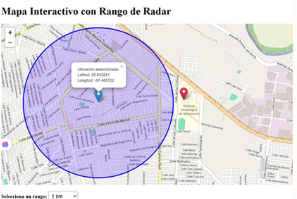
\includegraphics[width=15cm, height=11cm]{Pictures/mapa.png}
    \caption{Localizaciones}
\end{figure}


  
\vspace{3cm}



\chapter{Implementación de la interfaz (Pagina Web) }
\noindent
\section{Estructura del proyecto}
El proyecto \textbf{\textbf{"Educación Verde"}} es una página web diseñada para educar a los usuarios sobre el cuidado de árboles frutales. La página incluye secciones con consejos, guías, beneficios y características de diferentes árboles frutales. Además, utiliza Bootstrap para el diseño responsivo y JavaScript para generar contenido dinámico el proyecto está compuesto por los siguientes archivos:

\textbf{\subsection {Tecnologías Usadas}}
Archivo principal que contiene la estructura HTML de la página.

\textbf{1}  \textbf{\textbf{Encabezado (<header>)}}:

    Contiene el logo y el título de la página.
    
    Diseño responsivo con Bootstrap.\
    

\textbf{\textbf{HTML5}}: Para la estructura de la página.

\textbf{\textbf{CSS3}}: Para los estilos personalizados.

\textbf{\textbf{Tailwind css : }}Clases utilitarias predefinidas

\textbf{\textbf{JavaScript}}: Para generar contenido dinámico y manejar interacciones.

\textbf{\textbf{PostgreSQL}}: Sistema Gestor de Base de Datos para almacenar el contenido de la aplicación.

\textbf{\textbf{R2}}: Será usado para el almacenamiento de imágenes.

\textbf{\textbf{Imágenes}}: Utilizadas para ilustrar consejos, guías, beneficios y árboles frutales.

\vspace{5cm}

\section{Funcionalidades}

\subsection {Sección de consejos}
Muestra una lista de consejos para cuidar árboles frutales.
Cada consejo incluye una imagen, un título, una descripción breve y un botón "Leer más" que abre un modal con detalles adicionales.
\begin{figure}[H]
\centering
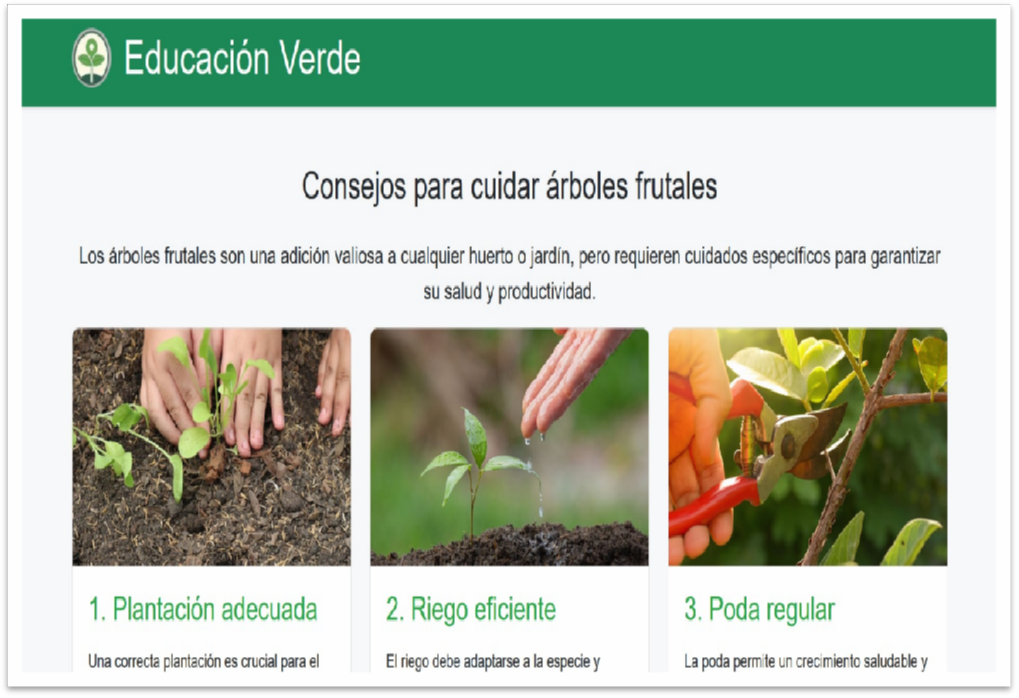
\includegraphics[width=0.8\textwidth]{Pictures/consejos.png}
\caption{Imagen de Consejos}
\end{figure}
\subsection {Sección de guías}
Proporciona guías prácticas para plantar y mantener árboles jóvenes.
Similar a la sección de consejos, incluye imágenes, títulos, descripciones y un botón para ver más detalles.
\begin{figure}[H]
\centering
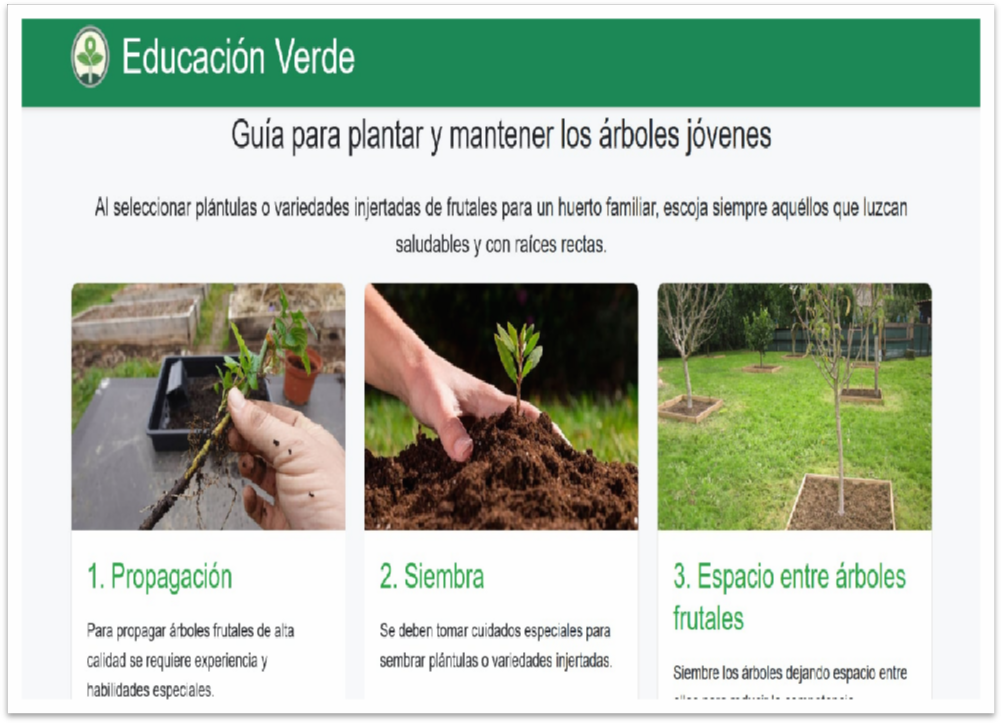
\includegraphics[width=0.8\textwidth, height=0.5\textwidth]{Pictures/guias.png}
\caption{Referencia del Radio de comunicación}
\end{figure}

\subsection { Sección de beneficios}
Enumera los beneficios de los árboles frutales para el medio ambiente.
Cada beneficio tiene una imagen y un botón para ver más información en el modal.
\begin{figure}[H]
\centering
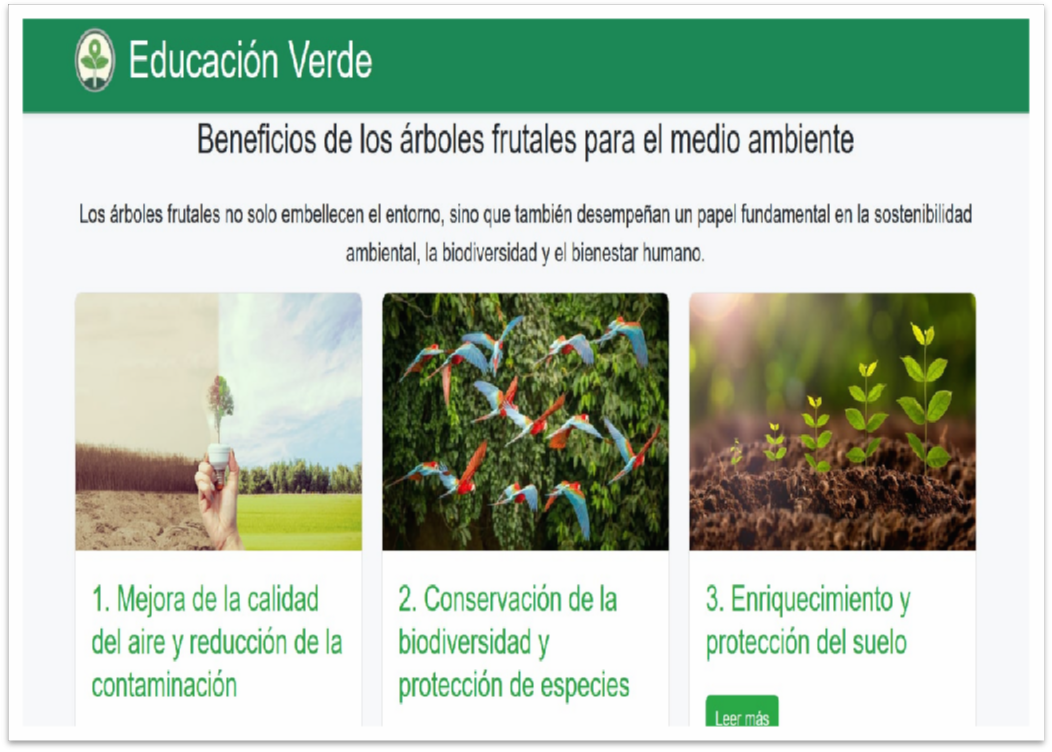
\includegraphics[width=0.75\textwidth]{Pictures/beneficios.png}
\caption{Referencia del Radio de comunicación}
\end{figure}
\subsection {Sección de árboles frutales}
Presenta una lista de árboles frutales con sus características, cuidados y recomendaciones de plantación.
\begin{figure}[H]
\centering
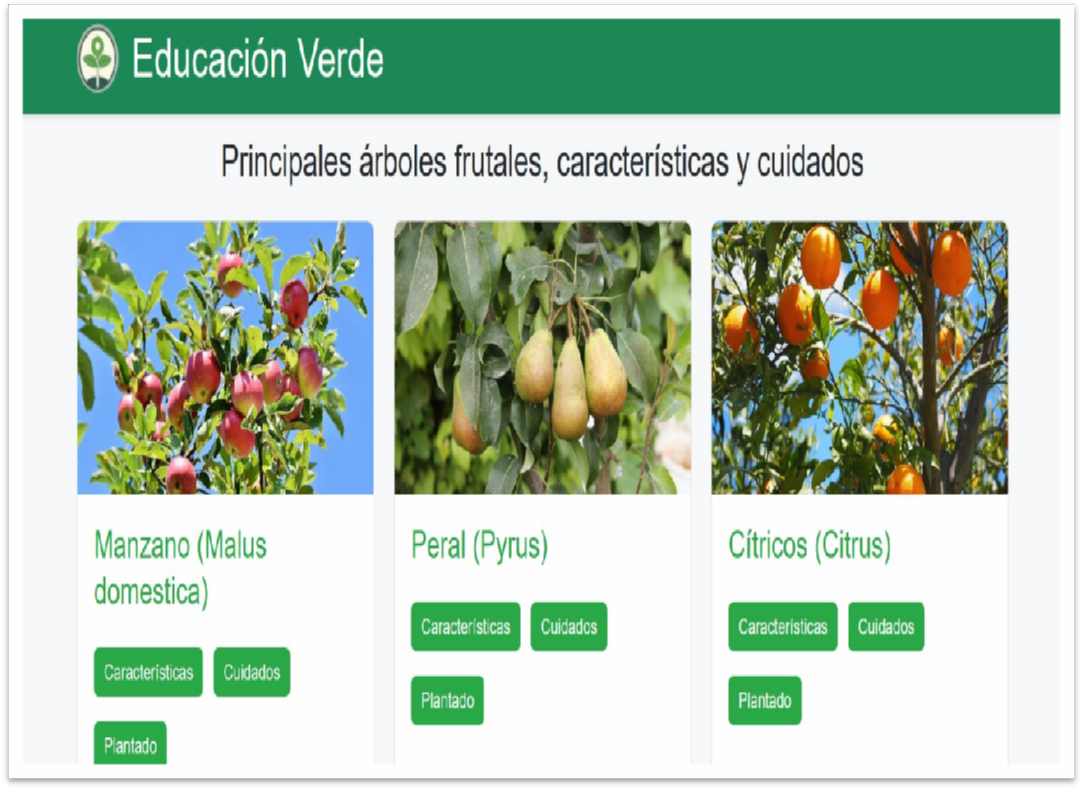
\includegraphics[width=0.8\textwidth]{Pictures/arboles.png}
\caption{Referencia del Radio de comunicación}
\end{figure}

Cada árbol tiene tres botones para ver detalles sobre sus características, cuidados y cómo plantarlo.
Beneficios
Enumera los beneficios de los árboles frutales para el medio ambiente.
Cada beneficio tiene una imagen y un botón para ver más información en el modal
\begin{figure}[H]
\centering
\includegraphics[width=1\textwidth]{Pictures/arbolbeneficios.png}
\caption{Referencia del model de beneficios}
\end{figure}

\subsection {Modal}
Un modal reutilizable que muestra información detallada dependiendo del botón que se haya hecho clic.
El contenido del modal se genera dinámicamente con JavaScript.
\begin{figure}[H]
\centering
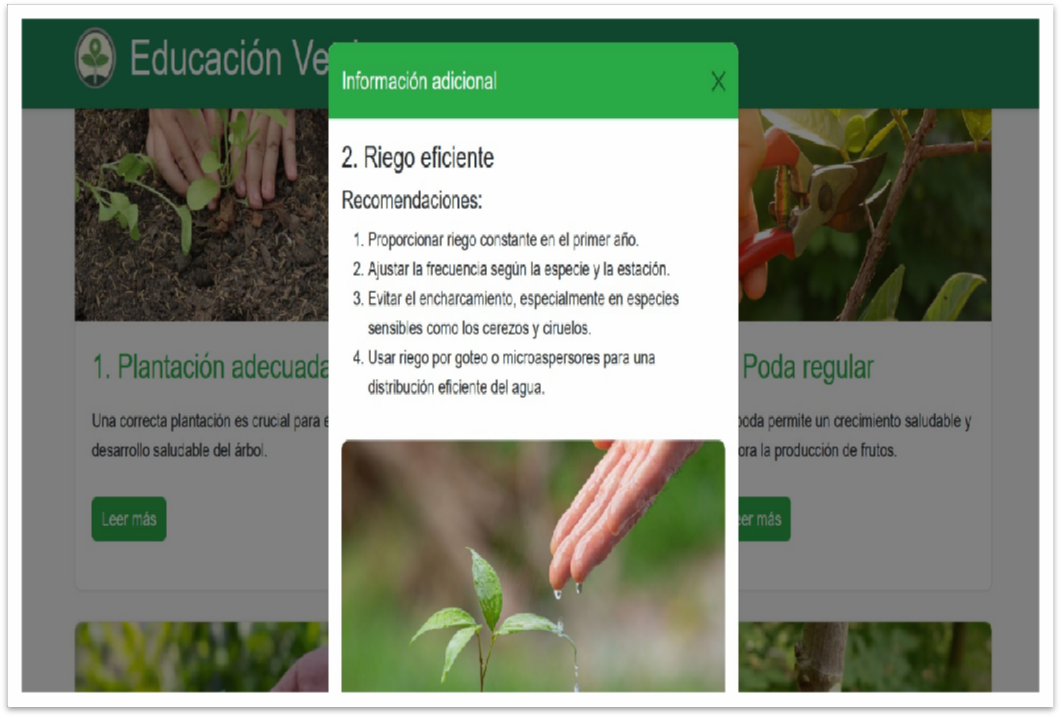
\includegraphics[width=0.9\textwidth]{Pictures/modal.png}
\caption{Referencia del Radio de comunicación}
\end{figure}
\vspace{3cm}
Los modales mejoran la experiencia de usuario al mostrar información detallada sin abandonar la página actual, manteniendo el contexto y la fluidez de navegación.
\begin{figure}[H]
\centering
\includegraphics[width=0.9\textwidth]{Pictures/experiencia.png}
\caption{Informacion adicional}
\end{figure}

\subsection {Comunidad}
Presenta publicaciones relacionadas a la temática. Dichas publicaciones son hechas por parte de los usuarios, donde cada publicación deberá contener: titulo, contenido, imagen y tema.
\begin{figure}[H]
\centering
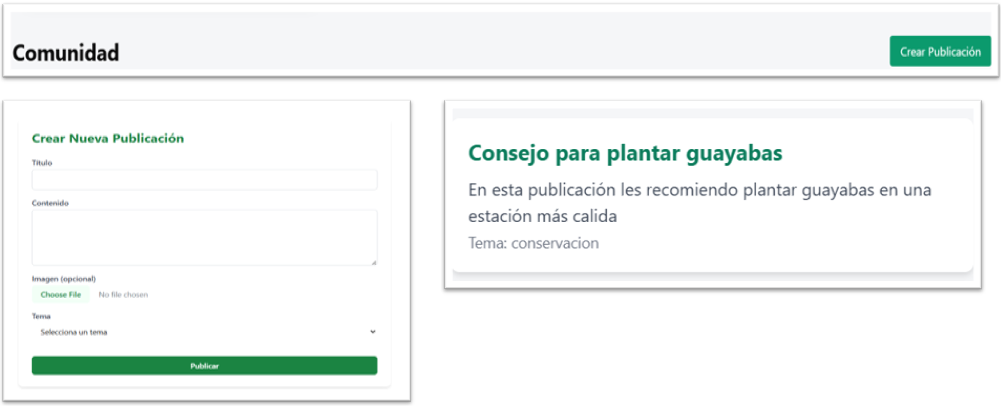
\includegraphics[width=1\textwidth]{Pictures/comunidad.png}
\caption{Visualización del apartado de Comunidad}
\end{figure}

\subsection{Base de Datos Versión Web}
La tabla de secciones será utilizada para filtrar las cartas o tarjetas dependiendo de su contenido. Las secciones serán especificadas más adelante en el documento. Esta tabla posee los siguientes atributos:

\begin{itemize}
    \item \textbf{id\_seccion (PK)}: Clave primaria, utilizada para identificar cada sección agregada.
    \item \textbf{nombre (varchar)}: Nombre de la sección, algunos ejemplos: “consejos”, “guías”, “beneficios”, etc.
    \item \textbf{descripción}: Breve descripción del contenido de cada sección.
\end{itemize}

\subsection{Base de Datos Modal}
La tabla de cartas será utilizada para almacenar la información de las tarjetas utilizadas para la visualización modal. La tabla posee los siguientes atributos:

\begin{itemize}
    \item \textbf{id\_carta (PK)}: Clave primaria que identifica cada tarjeta disponible en la aplicación.
    \item \textbf{id\_seccion (FK)}: Clave foránea que referencia la tabla \textbf{secciones}, utilizada para clasificar las tarjetas en sus respectivas secciones.
    \item \textbf{id\_usuario (FK)}: Clave foránea que referencia la tabla \textbf{usuarios}, permitiendo relacionar la tarjeta con el usuario creador.
    \item \textbf{titulo (varchar)}: Contiene el título de la tarjeta.
    \item \textbf{descripción (varchar)}: Contiene la información dentro de la tarjeta.
    \item \textbf{fecha (date)}: Almacena la fecha en la que se generó la tarjeta.
\end{itemize}


\begin{figure}[H]
\centering
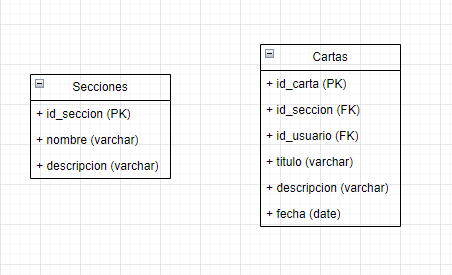
\includegraphics[width=0.8\textwidth]{Pictures/bd5.png}
\caption{Visualización del apartado de Comunidad}
\end{figure}

\chapter{Sistema de Reputación}

\section{Encuesta de Reputación}

Se diseñó la interfaz de la encuesta de reputación con la inclusión de imágenes gráficas representativas del nivel de satisfacción del usuario. Estas imágenes fueron integradas a la pantalla de evaluación para mejorar la experiencia visual y facilitar la comprensión del sistema de calificación.


\begin{figure}[H]
    \centering
    \begin{minipage}{0.45\textwidth}
        \centering
        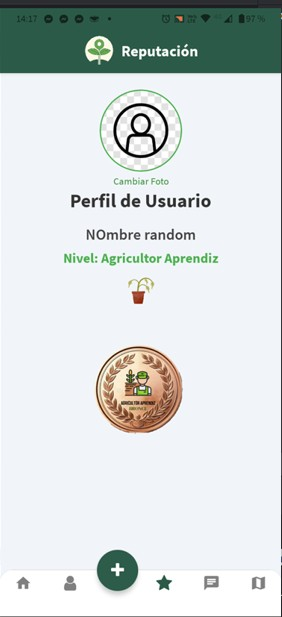
\includegraphics[width=5.5cm,height=11cm]{Pictures/reputacion7.jpg}
        \caption{Perfil de usuario.}
    \end{minipage}
    \hfill
    \begin{minipage}{0.40\textwidth} 
        \centering
        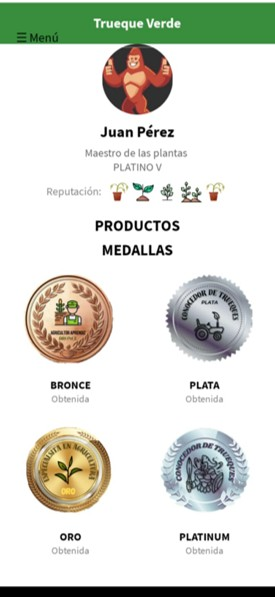
\includegraphics[width=5.5cm,height=11cm]{Pictures/reputacion6.jpg}
        \caption{Diseño de medallas.}
    \end{minipage}
\end{figure}

\section{Funcionalidad de Foto de Perfil}

Se habilitó una funcionalidad provisional para el cambio de foto de perfil. Al presionar la imagen actual, el sistema abre una ventana con los archivos locales del dispositivo, permitiendo al usuario seleccionar y recortar una nueva imagen. Esta funcionalidad se mantiene activa únicamente durante la sesión actual de ejecución.

\section{Elementos del Perfil de Usuario}

Se implementaron las siguientes características en la vista de perfil:

\begin{itemize}
    \item \textbf{Medallas:} Se muestran correctamente según el nivel de reputación del usuario. Al seleccionar una medalla, se despliega una descripción detallada del logro correspondiente.
    \item \textbf{Menú lateral:} Ubicado en la parte superior izquierda, permite acceso a funciones adicionales, como la activación del modo oscuro. El menú se despliega en la misma posición al ser presionado.
    \item \textbf{Nivel de reputación:} Visualizado mediante diseños representativos en forma de plantas, que indican el progreso del usuario.
    \item \textbf{Banner superior:} Se añadió un encabezado con el nombre del proyecto ``Trueque Verde'' para reforzar la identidad visual.
\end{itemize}

    \begin{figure}[H]
    \centering
    \begin{minipage}{0.45\textwidth}
        \centering
        
\includegraphics[width=6.5cm,height=14cm]{Pictures/reputacion4.jpg}
        \caption{alerta.}
    \end{minipage}
    \hfill
    \begin{minipage}{0.40\textwidth} 
        \centering
        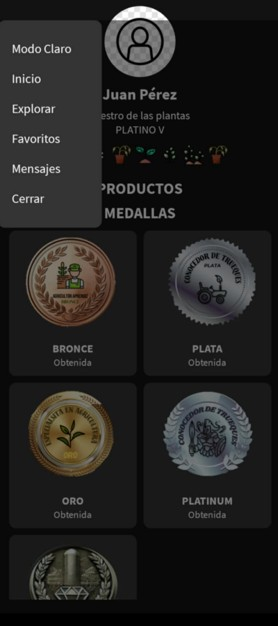
\includegraphics[width=6.5cm,height=14cm]{Pictures/reputacion5.jpg}
        \caption{menu lateral.}
    \end{minipage}
\end{figure}

\section{Integración del Sistema de Reputación}

El sistema de reputación fue integrado a la navegación principal del proyecto, permitiendo su acceso desde el resto de las pantallas. Se realizaron pruebas con diferentes usuarios, verificando lo siguiente:

\begin{itemize}
    \item Visualización correcta del nivel de reputación.
    \item Asignación automática de medallas (Bronce, Plata, Platino, Diamante) según el puntaje alcanzado.
    \item Presentación del título más alto logrado por el usuario.
    \item Actualización dinámica de la calificación global.
\end{itemize}

    \begin{figure}[H]
    \centering
    \begin{minipage}{0.45\textwidth}
        \centering
        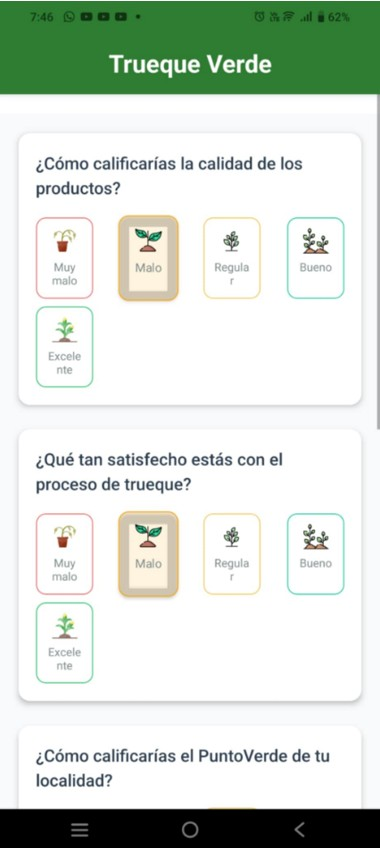
\includegraphics[width=6cm,height=13cm]{Pictures/reputacion1.jpg}
        \caption{alerta.}
    \end{minipage}
    \hfill
    \begin{minipage}{0.40\textwidth} 
        \centering
        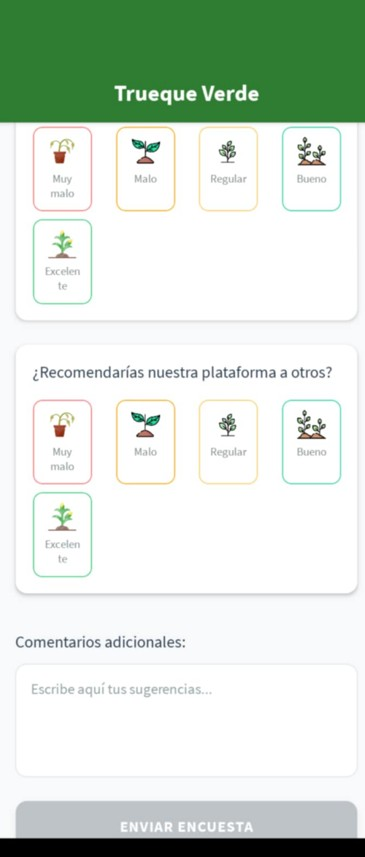
\includegraphics[width=6cm,height=13cm]{Pictures/reputacion2.jpg}
        \caption{menu lateral.}
    \end{minipage}
\end{figure}
\section{Comunicación Frontend–Backend}

Se resolvieron problemas de conexión entre la interfaz y el backend, permitiendo la extracción y visualización en tiempo real de los datos del usuario. Esto garantiza una sincronización efectiva del estado de reputación y los logros obtenidos.




\chapter{ Implementación de la interfaz del panel de administración }

El sistema de moderación de usuarios y publicaciones está diseñado para garantizar un entorno seguro dentro de la plataforma. Para ello, se han implementado funcionalidades que permiten la gestión de reportes, la revisión de publicaciones y la toma de decisiones sobre su estado.

\hspace{2cm}

Para optimizar el proceso de moderación, se han incorporado ventanas emergentes (modales) que muestran información detallada de cada reporte, incluyendo la fecha, el motivo y el usuario denunciante, además de opciones para tomar medidas directamente desde la interfaz.

\section{Usuarios Problemáticos }

Listado de Características y Funcionalidades del código,búsqueda de reportes tabla de usuarios responsable.


• Usuario reportado.

• Razón del reporte (ejemplo: "Contenido ofensivo").

• Cantidad de reportes recibidos.

• Estado del usuario. 

\hspace{6cm}

\section{Publicaciones } 

Este código implementa una página de administración para la moderación de publicaciones reportadas dentro de una plataforma. Su propósito es permitir que los
administradores revisen, aprueben o eliminen publicaciones que han sido reportadas por los usuarios. 



1-Filtros para Buscar Publicaciones Reportadas



• Pendiente de revisión" → No ha sido moderada aún. 


• "Eliminada" → Se consideró inadecuada y se borró.


• "Aprobada" → Se validó y es visible para los usuarios.


• Botón "Filtrar" para aplicar los criterios de búsqueda.

\section{Tabla de Publicaciones } 


• ID único de la publicación.

• Usuario que realizó la publicación.

• Razón del reporte (ejemplo: "Contenido ofensivo").

Estado actual de la publicación:

• Pendiente de revisión → Necesita ser moderada.

• Eliminada → Se eliminó por incumplimiento de normas.

• Aprobada con advertencia → Permitida, pero el usuario fue advertido.

Acciones disponibles para cada publicación:

• "Ver Detalles" → Muestra información completa de la publicación en un modal.

• "Advertir" → Envía una advertencia al usuario sobre su contenido.

• "Eliminar" → Elimina la publicación por incumplir normas.

• "Aprobar" → Permite que la publicación se mantenga visible. 

\section{Ventanas Emergentes (Modales) con Detalles de la Publicación} 

Usuario 1 tiene un modal con información detallada:

• Fecha del reporte: 21-02-2025.

• Razón: Contenido ofensivo.

• Reportado por: @usuarioReportadorX.

Contenido de la publicación:

• Imagen publicada (placeholder de imagen).

• Texto de la publicación, visible en un bloque de cita.

Acciones disponibles dentro del modal:

• Advertir al usuario sobre el contenido.

• Eliminar la publicación si infringe normas.

• Aprobar la publicación si no hay problemas.

\section{Panel de Administracion}     

El panel de la interfaz de usuario del panel de administracion se esta realizado en Tailwind y contiene lo siguiente: 

* Estadísticas de intercambios
\begin{figure}[H]
\centering
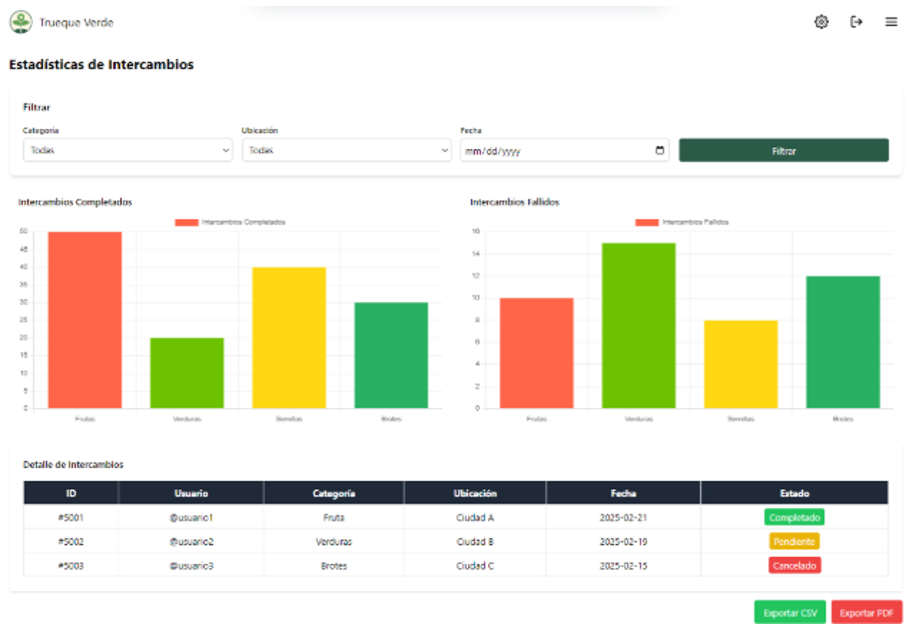
\includegraphics[width=0.73\textwidth]{Pictures/Imagen 8.png}
\caption{Visualización de Administracion}
\end{figure}
* Moderación de publicaciones
\begin{figure}[H]
\centering
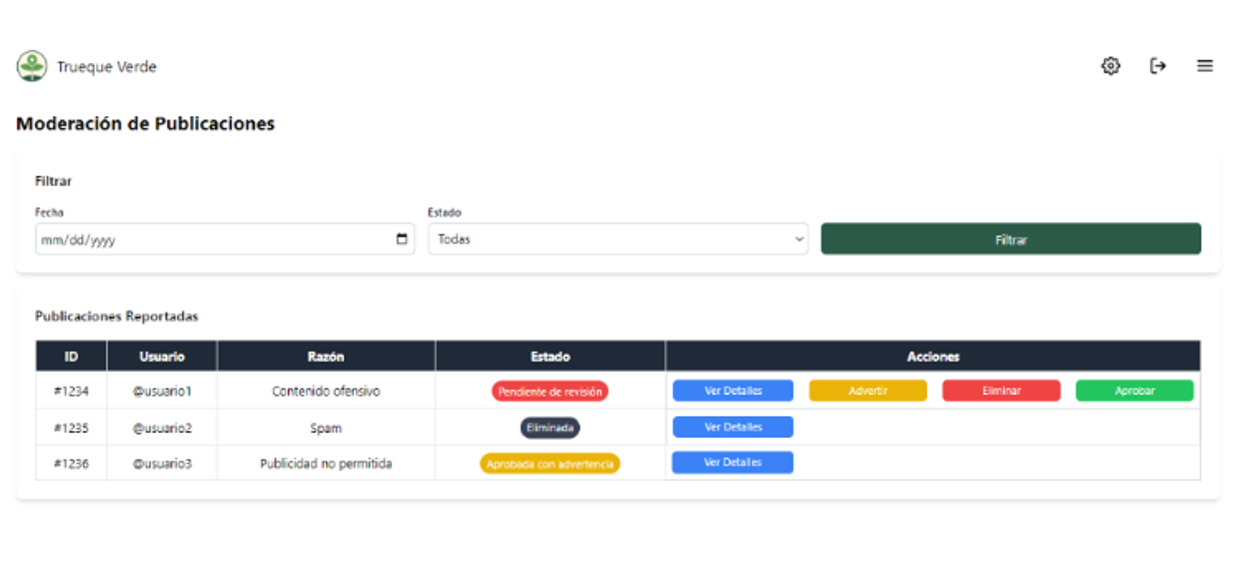
\includegraphics[width=0.8\textwidth]{Pictures/Imagen 9.png}
\caption{Visualización de la Moderacion}
\end{figure}
* Moderación de publicaciones nuevas
\begin{figure}[H]
\centering
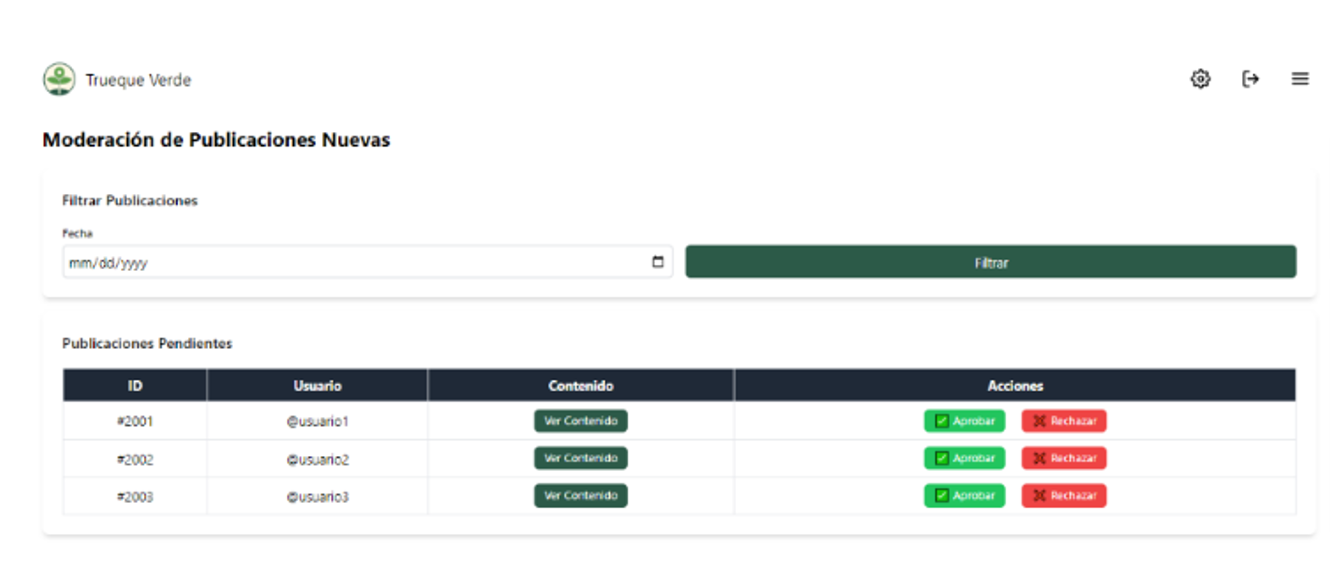
\includegraphics[width=0.8\textwidth]{Pictures/Imagen 10.png}
\caption{Visualización de moderación de entrada}
\end{figure}
* Administración de usuarios
\begin{figure}[H]
\centering
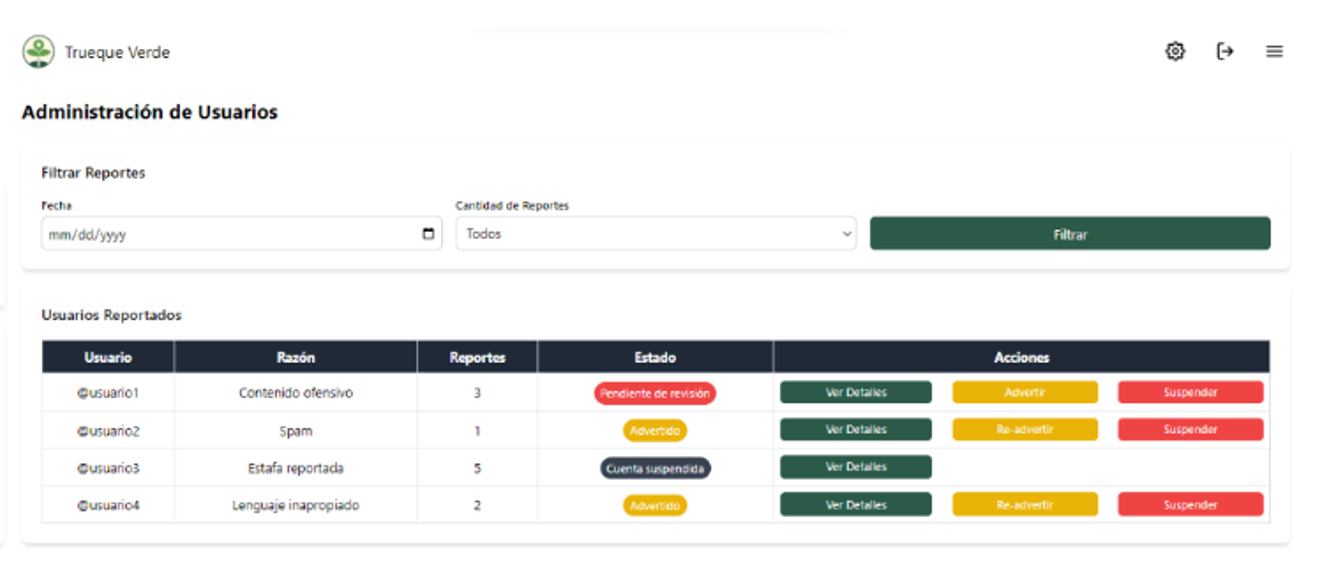
\includegraphics[width=0.8\textwidth]{Pictures/Imagen 11.png}
\caption{Visualización de la administrador de usuarios}
\end{figure}

\chapter{Equipos de Trabajos}

\section*{Equipo 1}
\begin{itemize}
    \item Isaac Segovia Cazares
    \item Johan Adrian Gonzalez Loza
    \item Felipe Jesus Hernandez Guzman
    \item Mauricio Eliseo Rosales Weigend
    \item Kevin del Angel Colunga Vazquez
    \item Santiago Emmanuel Garcia Villanueva
\end{itemize}

\section*{Equipo 2}
\begin{itemize}
    \item Camarillo Estrada Alonso Emmanuel
    \item González Rodríguez Kevin Eduardo
    \item Jiménez Reséndiz Karla Rebeca
    \item Muñoz Ordoñez José Daniel
\end{itemize}

\section*{Equipo 3}
\begin{itemize}
    \item Alcocer Rangel Fernando
    \item Del Angel Díaz Danniel Ehud
    \item López Nava Alejandro
    \item Lozano Velazquez Brandon Armando
    \item Torres Martínez José Francisco
    \item Ramos González Edgar Karol
\end{itemize}

\section*{Equipo 4}
\begin{itemize}
    \item Jan Karlo Armendariz Gonzalez
    \item Leslie Yiharem Aguirre Isassi
    \item Andrea Sordel Guzmán
    \item Jessica Rubi Gallegos Rodriguez
    \item Joel Sánchez Gutiérrez
    \item Fabiola de Jesus Cuellar Hiyan
\end{itemize}

\section*{Equipo 5}
\begin{itemize}
    \item Garibaldi Zúñiga, Daniel
    \item González Pérez, Erick Eduardo
    \item Herrera Galaviz, Leonardo
    \item Márquez Ruiz, José de Jesús
    \item Rivera Jaramillo, Jesús Naum
\end{itemize}

\section*{Equipo 6}
\begin{itemize}
    \item Padron Zaleta Jared Alfredo
    \item Patiño Herrera Edgar Ivan
    \item Perez Calderon Gerardo Adrian
    \item Lopez Cantu Andres Manuel
    \item Zaleta Diaz Dalia Nohemi
    \item Gutierrez Mendoza Osbel Emmanuel
\end{itemize}
\section*{Equipo 7}
\begin{itemize}
    \item Abellaneda Mejia Grecia Guadalupe
    \item Borjas Vega Gustavo Adrián 
    \item Flores Torres Jose Gerardo 
    \item Juárez Clemente Julio Antonio 
    \item Paz Miguel Angel
    \item Ramirez Reyes Eduardo 
\end{itemize}
\end{document}

\end{document}
